\chapter{Traitement d'images}

\lhead{\textit{Chapitre \thechapter}}
\rhead{\textit{Traitement d'images}}

\section{Introduction}
Lorem ipsum dolor sit amet, consectetur adipiscing elit. Curabitur a ullamcorper purus, sit amet cursus turpis. Nullam ipsum nibh, imperdiet vitae hendrerit et, porta sit amet lorem. In eu sem viverra, condimentum enim ac, congue dui. Quisque quis urna et quam vehicula tristique a a dui. Vestibulum euismod malesuada maximus. Vivamus vel lacinia nisi. Suspendisse ac fermentum ante, vel condimentum odio. Praesent ut nibh tempor, condimentum eros sit amet, scelerisque sapien. Nam ut nisl sit amet risus viverra fringilla quis a sapien. Curabitur id quam nisl. Sed volutpat varius neque eget tempor. Proin eget ultrices magna, ullamcorper ultricies leo. Suspendisse vitae ex sit amet dolor venenatis imperdiet non sit amet turpis. Vestibulum ante ipsum primis in faucibus orci luctus et ultrices posuere cubilia curae; Nulla quis suscipit ipsum. In rhoncus urna a quam eleifend, vitae euismod tellus varius.
\newpage
\section{Images numériques}
Maecenas vel condimentum lorem. Aenean a enim risus. Quisque quam orci, luctus at nibh eget, egestas tincidunt libero. Donec ultrices arcu neque, sed euismod augue porta ac. Vivamus mollis nisi elit, a facilisis tortor lobortis at. Donec rhoncus at leo id mollis. Cras porta purus eget diam ultrices, in accumsan eros faucibus. Nunc id vestibulum urna. Integer lobortis mauris vitae ligula ultricies, ut molestie odio sagittis. 


Pour un informaticien, une image est un type, une structure de données, qu'il appelle aussi structure de données maillées. Les images usuelles (celles qui peuvent être lues par un logiciel du commerce) s'appuient sur un support $\mathcal{D}$ dont la topologie est un maillage carré 2D régulier \cite{Guigues2003ModlesMP}:
\begin{equation}
\mathcal{D} = \lbrack 0,C\rbrack\times\lbrack 0,L\rbrack \footnote{Nous notons que, C = nombre de colonnes et L = nombre de lignes}
\end{equation}
\myequations{Image en forme mathématique}
\begin{figure}[htp]
    \centering
    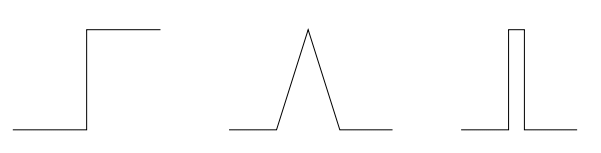
\includegraphics[width=11cm]{Chapiters/Chapiter_01/Pictures/Differents-types-de-contours-marche-descalier-toit-et-pointe.png}
    \caption{image caption.}
    \label{}
\end{figure}

\section{Conclusion}
Sed blandit, diam ut mollis vehicula, tortor mi efficitur dui, quis suscipit mauris velit quis urna. Mauris et ullamcorper augue. Suspendisse nulla est, elementum quis leo a, faucibus convallis lorem. Suspendisse tempor consequat tortor. Maecenas ornare non felis non mattis. Aenean facilisis convallis nisi. Duis mollis nisl vitae aliquam malesuada. Vestibulum eu egestas neque. Fusce ac justo risus. Pellentesque tempus eros non rhoncus condimentum. Aenean pulvinar tristique orci feugiat bibendum. Donec suscipit sem nec massa ultricies tristique sed at tortor. Nulla facilisi. Morbi ut arcu consectetur, hendrerit odio nec, ornare urna. Nunc ac feugiat orci, eget auctor sapien.
      



